\section{Exploring the Schedule Space}
\label{sec:exploring}

% \begin{itemize}
%   \item The scheduling language described in Section \ref{sec:schedule} allows
%   for numerous possible schedules for a given model. 
%   Finding a schedule with good performance is a non-trivial task.
%   \item We identify a reasonable template schedule for GPUs which encompasses
%   all strategies published in prior work.
%   \item Describe the template schedule.
%   \item Even within the variants of this template schedule, there is a significant 
%   amount of variation in performance. Show the histogram. 
%   \item Extensively exploring all possible parameter values for the template schedule 
%   is infeasible due to the large number of parameters.
%   Cite some numbers on how long it takes to explore the schedule space.
%   \item List the observations we make and the heuristic we design based on these.
% \end{itemize}

The set of schedules that can be constructed using the scheduling language described in 
Section \ref{sec:schedule} is unbounded. Searching this schedule space to find a 
high-performance schedule is a non-trivial task. To simplify this process, we design a
template schedule for GPUs that encompasses several strategies published in prior work.
Our template schedule assigns a configurable number of rows to each thread block and to each thread.
It distributes the trees across a specified number of threads and can cache trees and 
input rows if required while unrolling and interleaving of tree walks.
Table \ref{tab:schedparams} lists the parameter values we tried. 
% \begin{itemize}
%   \item \textbf{Number of rows per thread block (Integer):} The number of rows that are processed by each thread block.
%   \item \textbf{Number of rows per thread (Integer):} The number of rows processed by each thread.
%   \item \textbf{Number of tree threads (Integer):} The number of threads across which the trees are distributed.
%   \item \textbf{Cache rows (Boolean):} Whether the input rows are cached in shared memory.
%   \item \textbf{Cache trees (Boolean):} Whether the trees are cached in shared memory.
%   \item \textbf{Unroll walks (Boolean):} Whether the tree walks are unrolled.
%   \item \textbf{Tree walk interleave factor:} The number of tree walks that are interleaved.
%   \item \textbf{Shared memory reduction:} Whether the reduction across tree threads is done in shared memory.
% \end{itemize}

\begin{table}[htb]
  \centering
  \resizebox{\linewidth}{!}{
  \begin{tabularx}{\linewidth}{c | c }
  \toprule
  \textbf{Parameter} & \textbf{Values} \\
  \midrule
  \textbf{Rows per thread block} & $\{8, 32, 64\}$ \\
  \textbf{Rows per thread} & $\{1, 2, 4\}$ \\
  \textbf{Number of tree threads} & $\{2, 10, 20, 50\}$ \\
  \textbf{Cache rows} & $\{True, False\}$ \\
  \textbf{Cache trees} & $\{True, False\}$ \\
  \textbf{Unroll walks} & $\{True, False\}$ \\
  \textbf{Tree walk interleave factor} & $\{1, 2, 4\}$ \\
  \textbf{Shared memory reduction} & $\{True, False\}$ \\
  \bottomrule
  \end{tabularx}
  }
  \vskip 5pt
  \caption{\label{tab:schedparams} List of parameter values we explored for the template GPU schedule.}
\end{table}

%While the template schedule simplifies optimization of generated inference code,
It is important to note that the \Treebeard{} compiler itself does not place any 
restrictions on the schedule. The user is free to specify any schedule they wish.
The compiler pass that implements the template schedule is also implemented as a 
module outside the core \Treebeard{} compiler. 
% Users are also free to implement 
% other auto-schedulers that generate schedules different from the template schedule.

\begin{figure}[htb]
  \centering
  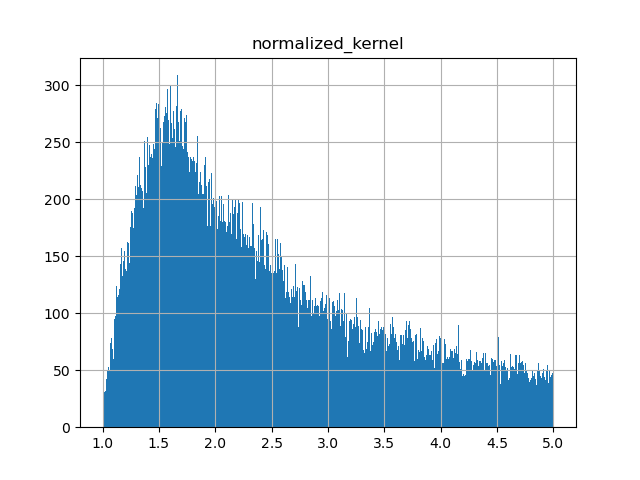
\includegraphics[width=\linewidth]{figures/normalized_kernel_histogram_lt5.png}
  \caption{Distribution of normalized execution times for all benchmark models
  with the template schedule using parameter values as shown in Table \ref{tab:schedparams}}. 
  \label{Fig:ExecTimeDistribution}
\end{figure}

While the template schedule simplifies code generation, finding a good set of 
parameter values is still hard.
Figure \ref{Fig:ExecTimeDistribution} shows the distribution of normalized execution times
for all benchmark models with different parameter values for the template schedule (inference
times normalized w.r.t fastest time for that model).
There is a significant amount of variation in performance even within the variants of the
template schedule,. Very few schedules perform close to the best while a vast majority of
schedules perform poorly.

Exploring the schedule space extensively even for a reasonable set of parameter values
is very expensive. We explored the set of parameter values listed in Table \ref{tab:schedparams}
for our benchmarks and found that it took anywhere between thirty minutes up to a few hours
to explore the entire space for each model. 
%Performing this extensive search for every model being compiled is infeasible in practise. 
We therefore
%need a better mechanism to guide the search for a good schedule.
design a heuristic to narrow down the set of schedules to explore based on the following 
observations.
\begin{itemize}
  \item For small batch sizes, the best schedules tend to have a small number of rows
  per thread block and partition the trees across a larger number of threads. This is 
  intuitive since the amount of data parallelism across the rows is limited for small batch sizes.
  \item Always cache rows in shared memory and never cache trees. We find that caching rows 
  %when possible (i.e., when the number of features is small enough to fit in shared memory)
  almost always improves performance. Caching trees on the other hand almost always degrades 
  performance. This is because the one time cost of loading trees into shared memory is 
  not sufficiently amortized when the whole of the tree is not accessed during inference. 
  \item Models with a large number of features tend to benefit from partitioning the 
  trees across more threads even at larger batch sizes. This is because processing fewer rows at a time 
  allows us to keep them in shared memory.
  % We empirically find that the threshold for when 
  % we should start partitioning the trees across more threads is when the number of features
  % is greater than 100. 
  \item We find that when a model prefers schedules with shared reduction, the same schedules 
  without shared reduction are among the best performing schedules without shared reduction.
  % We therefore are able to separate the evaluation of shared reduction by collecting the 
  % best schedules without shared reduction and only evaluating shared reduction on them. 
  Evaluating the top 3 schedules for shared reduction is sufficient in practice.  
\end{itemize}

\Treebeard{} uses these observations to narrow down the set of schedules to explore. 
The pseudo-code for the heuristic is shown in Algorithm \ref{alg:heuristic}.
The algorithm first computes a subset of thread block configurations in the function 
\op{TBConfigs}. A set of schedules based on these thread block configurations 
is then computed (\op{schedules}). The model is compiled with each of these schedules 
and then the resulting inference code is profiled. The three best performing schedules 
are collected and shared reduction is enabled on them and the resulting schedules evaluated.
The best schedule among all the evaluated schedules is selected as the schedule to use.
We find that this heuristic is able to find schedules that are close to the best schedules
but improves the search time by two orders of magnitude as we show in Section \ref{sec:results}.

\begin{algorithm}
  \caption{Heuristic to find a good schedule}
  \label{alg:heuristic}
  \begin{algorithmic}[1]
  \Procedure{TBConfigs}{$N_{batch}$, $N_f$}
    \State $T_{batch} \gets 2048,\; T_f \gets 128$
    \If {$N_{batch} \leq T_{batch}$ \textbf{or} $N_{f} > T_{f}$}
      \State $rowsPerBlock \gets \{8, 32\}$
      \State $treeThreads \gets \{20, 50\}$
    \Else
      \State $rowsPerBlock \gets \{32, 64\}$
      \State $treeThreads \gets \{2, 10\}$
    \EndIf
    \State \Return $rowsPerBlock, treeThreads$
  \EndProcedure
  \\
  \State $bestSchedules \gets shMemSchedules \gets \emptyset$
  \State $rowsPerTB, treeThds \gets TBConfigs(N_{batch}, N_f)$
  \State $cacheRows \gets \text{True},\; cacheTrees \gets \text{False}$
  \State $interleave \gets \{1, 2, 4\}$
  % \State $reps \gets \{array, sparse, reorg\}$
  \State $schedules \gets (rowsPerTB, treeThds, cacheRows,$ \\
                          \hspace{2cm}$cacheTrees, interleave)$
                          %\hspace{2cm}$$
  \For{$(sched, rep) \in schedules \times \{array, sparse, reorg\}$}
    \State $time \gets EvaluateSchedule(sched, rep)$
    \State $bestSchedules.insert(time, sched, rep)$
  \EndFor
  \State 
  \For{$sched, rep \in Top3(bestSchedules)$}
    \State $EnableSharedReduction(sched)$
    \State $time \gets EvaluateSchedule(sched, rep)$
    \State $shMemSchedules.insert(time, sched, rep)$
  \EndFor
  \State \Return $min(shMemSchedules \cup bestSchedules)$
  \end{algorithmic} 
\end{algorithm}